\documentclass[compress]{beamer}
\usepackage[latin1]{inputenc}
%\usepackage[pdftex]{graphicx}
\usepackage{alltt}
\title{Root Isolation for one-variable polynomials}
\author{Yves Bertot\\
{\em Joint work with}\\ Assia Mahboubi and Fr�d�rique Guilhot}
\date{July 2010}
\begin{document}
\maketitle
\begin{frame}
\frametitle{Introduction}
\begin{itemize}
\item Solving systems of inequations and geometrical problems
\item Does there exist \((x,y)\) so that the following comparisons hold?
\begin{eqnarray*}x^2 &\leq& y\\
y &\leq& 18 - 3 x + 9 x^2\\x &<& 1
\end{eqnarray*}
\item Here find whether the roots of \(18 -3 x + 10 x^2\) are in some interval.
\item More general applications in quantifier elimination and
cylindrical decomposition
\item Can be used to define algebraic numbers
\end{itemize}
\end{frame}
\begin{frame}
\frametitle{Method}
\begin{itemize}
\item Bernstein coefficient approximate a polynomial's curve
\item Discrete approximation
\begin{itemize}
\item Associated to bounded intervals
\end{itemize}
\item Exactly one sign change implies exactly one root in the interval
\item No sign change implies no root in the interval
\begin{itemize}
\item More than one sign change: no conclusion
\end{itemize}
\item Refinement: cut the interval in halves and start again
\begin{itemize}
\item Use a simple combinatorial algorithm
\end{itemize}
\end{itemize}
\end{frame}
\begin{frame}
\frametitle{Geometric intuition: Bernstein}
\begin{center}

\includegraphics[clip=true,scale=0.4,trim=2cm 4cm 1cm 6.3cm]{control.pdf}
\end{center}
\end{frame}
\begin{frame}
\frametitle{Geometric intution: False alert}
\begin{center}

\includegraphics[clip=true,scale=0.4,trim=2cm 4cm 1cm 6.3cm]{control2.pdf}
\end{center}
\end{frame}
\begin{frame}
\frametitle{Geometric intution: Exactly one root}
\begin{center}

\includegraphics[clip=true,scale=0.4,trim=2cm 4cm 1cm 6.3cm]{control3.pdf}
\end{center}
\end{frame}
\begin{frame}
\frametitle{Geometric intuition: interval splitting}
\begin{center}

\includegraphics[clip=true,scale=0.4,trim=2cm 4cm 1cm 6.3cm]{control4.pdf}
\end{center}
\end{frame}
\begin{frame}
\frametitle{Computing Bernstein coefficients}
\begin{itemize}
\item Polynomial \(a_0 + a_1 X + \cdots + a_n X^n\)
\item Bernstein coefficients for interval \((l,r)\)\\
\[b_i =\sum_{j=0}^n \left(\begin{array}{c}j\\n\end{array}\right)
a_i\frac{r^j l^{n-j}}{r-l}\]
\item Easy computation of Bernstein coefficients for the half intervals
\begin{itemize}
\item de Casteljau's algorithm
\end{itemize}
\end{itemize}
\end{frame}
\begin{frame}
\frametitle{Correctness proof}
\begin{itemize}
\item Relate Bernstein coefficients with plain coefficients of another
polynomial
\begin{itemize}
\item Using an automorphism
\end{itemize}
\item Prove Descartes' law of signs (on a simple case)
\item Establish correspondances between the roots of both polynomials
\item Make the combinatorial proof for interval splitting
\end{itemize}
\end{frame}
\begin{frame}
\frametitle{Constructive proof}
\begin{itemize}
\item Use rational numbers
\item New meaning of ``having a root''
\item Decompose interval into several parts
\begin{itemize}
\item parts where the absence of root is guaranteed
\item parts where the polynomial changes sign, with monotonicity
\end{itemize}
\item Replacement for the intermediate value theorem
\begin{itemize}
\item Express that one can find a value that is arbitrary close to 0.
\item Upper bound on slopes for polynomials and bounded intervals
\item Deduce uniform continuity
\item take regularly spaced points and work in a discrete setting
\end{itemize}
\end{itemize}
\end{frame}
\begin{frame}
\frametitle{Sufficient conditions for one root only}
\begin{center}

\includegraphics[clip=true,trim= 2cm 7cm 0cm 9cm,scale=0.3]{bounded_decompose.pdf}
\end{center}
\end{frame}
\begin{frame}
\frametitle{Sufficient conditions for one root only}
\begin{center}

\includegraphics[clip=true,trim= 2cm 4cm 0cm 9cm,scale=0.3]{unbounded_decompose.pdf}
\end{center}
\end{frame}
\begin{frame}
\frametitle{Intermediate value theorem replacement}
\begin{itemize}
\item The intermediate value theorem is used to produce a root
\item Here, we only want to use to produce a two values \(x'\) and \(y'\)
\begin{itemize}
\item The polynomial in these two values is close enough to 0
\item The polynomial is negative in \(x'\) and positive in \(y'\)
\end{itemize}
\item Proof using an upper bound on slopes
\end{itemize}
\end{frame}
\begin{frame}
\frametitle{Intermediate value theorem replacement}
\begin{center}

\includegraphics[clip=true,trim=0cm 9cm 2cm 9cm,scale=0.5]{ivt.pdf}
\end{center}
\end{frame}
\begin{frame}
\frametitle{Descartes' law of signs}
\begin{itemize}
\item A relation between sign changes and the number of positive roots
\item \textcolor{blue}{The number of changes is larger than the number of roots}
\begin{itemize}
\item More precisely, the difference is a multiple of 2
\item Counting multiplicity of roots
\end{itemize}
\item \((x - 1) * (x ^ 2 + 2) = x^3 + x^2 -2\) : 1 sign change
\item \((x - 1)^2 = x ^2 -2 x + 1\) : 2 sign changes
\item \((x - 1) (x - 2) = x ^2 -3 x + 2\) : 2 sign changes
\item If there is exactly one sign change, there is exactly one root
\begin{itemize}
\item A specific proof for this corollary
\end{itemize}
\end{itemize}
\end{frame}
\begin{frame}
\frametitle{Proving Descartes' corollary}
\begin{itemize}
\item A finite state approach
\item five kinds of polynomial curves,
\item move from one kind to the other by apply Horner's scheme
\item move depends on the sign of the added constant.
\end{itemize}
\end{frame}
\begin{frame}
\frametitle{Geometric intuition for Descartes' corollary}
\begin{center}
\includegraphics[width=0.5\textwidth]{alternated2.png}
\end{center}
\end{frame}
\begin{frame}
\frametitle{More on Descartes}
\begin{itemize}
\item Use interval decompositions,
\item Assume \(P\) has a slope larger than \(k > 0\) above a bound \(y\)
\item When multiplying by \(X\), new slope is \(k x + P(x)\)
\item Use intermediate value replacement to make \(P(x)\) negligible
\item in a closed field we would simply use the existing root
\item When adding a negative constant \(a\), take a value so that 
\(0 \leq P(x) < P(a)\)
\end{itemize}
\end{frame}
\begin{frame}
\frametitle{From Bernstein to Descartes}
\begin{itemize}
\item Reversing the list of coefficients: nice trick!
\item \(P = rev(R) \Leftrightarrow P(x) = 1/x^n R(1/x)\)
\item Root of \(P\) in \((0,1)\) correspond to roots of \(R\) in
\((1,+\infty)\)
\item \(R'(x) = R(1 + x)\) and use Descartes' corollary for \(R'\)
\item For an arbitrary interval \((l,r)\), use change of variable\\
\(y = r x + (1 - x) l\)
\end{itemize}
\end{frame}
\begin{frame}
\frametitle{Difficulties in formalization}
\begin{itemize}
\item relate the slopes of \(P\) \(P(1/x)\) and \(R\)
\item Also use upper bounds of slopes
\end{itemize}
\end{frame}
\begin{frame}
\frametitle{Interval splitting}
\begin{itemize}
\item Remember Bernstein coefficients are obtained after translating,
flipping, and affine variable change
\item All linear invertible operations
\item Call \(v\) the vector of Bernstein coefficients
\item Call \(\phi\) the function so that \(\phi(p) = v\)
\item \(\phi\) can also be seen as function mapping polynomials to polynomials
\item consider \(P'_b(n, l, r, k)\) the inverse image of \(X^k\)
\item \(phi(p)= \sum_{k=0}^{n} v_i X^k \Leftrightarrow 
p = \sum_i v_i (P'_b(n,l,r,k))\)
\item Bernstein coefficients are coefficients in a precise basis
\item \(P_b(n, l, r, k) = \left(\begin{array}{c}k\\n\end{array}\right)
        x^{n-k}(1-x)^k\)
\end{itemize}
\end{frame}
\begin{frame}[fragile]
\frametitle{Combinatorial computation}
\begin{alltt}
Variables l r : Qcb.

Fixpoint dc (b : nat -> Qcb) (n : nat) :=
  if n is i.+1 then
     fun j => l * dc b i j + r * dc b i j.+1
   else b.

Definition dicho' b i := de_casteljau b i 0.
Definition dicho p b i := de_casteljau b (p - i) i.
\end{alltt}
\end{frame}
\begin{frame}
\frametitle{On Casteljau's algorithm}
\begin{itemize}
\item Algorithm due to P. de Casteljau (work on CAD)
\item Same scheme as for binomial coefficients
\item Combinatorial proof, relying on the Bernstein basis
\end{itemize}
\end{frame}
\begin{frame}
\frametitle{Conclusion}
\begin{itemize}
\item Basic blocs for a decision procedure
\item Start with an large bounded interval
\item Apply dichotomy until 0 or 1 alternation in Bernstein coefficients
\item Termination not proved yet (one known proof, using complex numbers)
\item First proofs done with real numbers (not maintained)
\item More recent proofs redone with {\tt ssreflect}
\end{itemize}
\end{frame}
\end{document}
%%% Local Variables: 
%%% mode: latex
%%% TeX-master: t
%%% End: 
